% ============================================================
%  Semana 8 · Clase 15: Identificación de insights (cont.)
%  Curso: Análisis y Visualización de Datos para la Toma de Decisiones
%
%  Formato de la sesión (3 h), en forma de guía paso a paso:
%    Hora 1. Medidas que responden a los filtros, metas y KPI
%    Hora 2. Segmentadores, filtros y jerarquías
%    Hora 3. Interacción entre objetos visuales y diseño de una página
%            orientada a preguntas de negocio
%
%  Datos: datos/gimnasio_vitalis.xlsx (el mismo archivo de las Clases 13
%  y 14, generado con ../../../scripts/semana07-clase13_datos.py)
%
%  Las capturas de figuras/ms-learn/ provienen de Microsoft Learn y se
%  usan sin modificar, según la política de Microsoft para capturas de
%  pantalla de sus productos ("Used with permission from Microsoft").
%
%  Compilar (dos veces) directamente desde esta carpeta:
%    xelatex semana08-clase15.tex
%    xelatex semana08-clase15.tex
% ============================================================
\documentclass[aspectratio=169,11pt]{beamer}

\usepackage{../../../plantilla/beamerthemeesumer}
\usetheme{esumer}

\usepackage[spanish,es-noshorthands]{babel}
\usepackage{booktabs}
\usepackage{graphicx}
\usepackage{array}
\newcolumntype{L}[1]{>{\raggedright\arraybackslash}p{#1}}
\usetikzlibrary{arrows.meta,positioning,calc}

% ---------------- DATOS DE LA CLASE ----------------
\title{Identificación de insights: KPI, segmentadores y filtros}
\subtitle{Guía paso a paso con los datos del Gimnasio Vitalis}
\author{Docente: Cristian A. Jimenez C., MSc}
\date{Oct 27 al 1 Nov}

\setmodulo{Módulo 3: Experimentar (Visualización e Insights)}
\setsemana{8}
\setclase{15}
\setfechaclase{Oct 27 al 1 Nov}
\setmodalidad{Virtual}
% -----------------------------------------------------

\graphicspath{{figuras/}}

% Pie de cada captura: producto, página de origen y la frase que exige Microsoft
\newcommand{\fuente}[2]{%
  \par\vspace{1pt}{\fontsize{5.5}{6.5}\selectfont\color{black!55}%
  Captura de Microsoft Power BI Desktop. Guía oficial de este paso:
  \href{#2}{\color{esumerOrange}«#1»}. Used with permission from Microsoft.\par}}

% Pie para los pasos sin captura: solo el enlace a la guía oficial
\newcommand{\guia}[2]{%
  \par\vspace{1pt}{\fontsize{6}{7}\selectfont\color{black!55}%
  Guía oficial de este paso: \href{#2}{\color{esumerOrange}«#1»}.\par}}

% Número de paso
\newcommand{\npaso}[1]{\tikz[baseline=(n.base)]\node[circle,fill=esumerOrange,
  text=white,font=\bfseries\footnotesize,inner sep=0pt,minimum size=0.48cm](n){#1};}

% Fórmula DAX en un recuadro sin título
\newcommand{\codigo}[1]{\par\smallskip\noindent\colorbox{esumerGray!70}{\parbox{\dimexpr\linewidth-2\fboxsep\relax}{\scriptsize\ttfamily #1}}\par\smallskip}

% Menú de Power BI: nombre en español (nombre en inglés)
\newcommand{\menu}[2]{\textbf{#1} {\color{black!55}(#2)}}

\newcommand{\urlinstalar}{https://learn.microsoft.com/es-es/power-bi/fundamentals/desktop-get-the-desktop}
\newcommand{\urlstore}{https://apps.microsoft.com/detail/9ntxr16hnw1t?hl=es-co}
\newcommand{\urlcentro}{https://www.microsoft.com/download/details.aspx?id=58494}
\newcommand{\urldatos}{https://github.com/craljimenez/An-lisis_y_Visualizacion_de_Datos_para_la_Toma_de_Decisiones/raw/main/clases/semana08-clase15-identificacion-insights-kpi-filtros/datos/gimnasio_vitalis.xlsx}
\newcommand{\urlmedidas}{https://learn.microsoft.com/es-es/power-bi/transform-model/desktop-measures}
\newcommand{\urlrapidas}{https://learn.microsoft.com/es-es/power-bi/transform-model/desktop-quick-measures}
\newcommand{\urlkpi}{https://learn.microsoft.com/es-es/power-bi/visuals/power-bi-visualization-kpi}
\newcommand{\urltarjeta}{https://learn.microsoft.com/es-es/power-bi/visuals/power-bi-visualization-card}
\newcommand{\urlsegmentadores}{https://learn.microsoft.com/es-es/power-bi/visuals/power-bi-visualization-slicers}
\newcommand{\urlsegvisual}{https://learn.microsoft.com/es-es/power-bi/visuals/power-bi-visualization-slicer-visual}
\newcommand{\urlsegjerarquia}{https://learn.microsoft.com/es-es/power-bi/create-reports/power-bi-slicer-hierarchy-multiple-fields}
\newcommand{\urlfiltros}{https://learn.microsoft.com/es-es/power-bi/create-reports/power-bi-report-add-filter}
\newcommand{\urltiposfiltros}{https://learn.microsoft.com/es-es/power-bi/create-reports/power-bi-report-filter-types}
\newcommand{\urlformatofiltros}{https://learn.microsoft.com/es-es/power-bi/create-reports/power-bi-report-filter}
\newcommand{\urlinteracciones}{https://learn.microsoft.com/es-es/power-bi/create-reports/service-reports-visual-interactions}
\newcommand{\urlexplorar}{https://learn.microsoft.com/es-es/power-bi/explore-reports/end-user-drill}
\newcommand{\urltutorial}{https://learn.microsoft.com/es-es/power-bi/create-reports/desktop-dimensional-model-report}
\newcommand{\urltrucos}{https://learn.microsoft.com/es-es/power-bi/create-reports/desktop-tips-and-tricks-for-creating-reports}
\newcommand{\urlcuadricula}{https://learn.microsoft.com/es-es/power-bi/create-reports/desktop-gridlines-snap-to-grid}
\newcommand{\urltemas}{https://learn.microsoft.com/es-es/power-bi/create-reports/desktop-report-themes}

\begin{document}

{
\setbeamertemplate{footline}{}
\begin{frame}[plain,noframenumbering]
  \titlepage
\end{frame}
}

\begin{frame}[t]{Agenda de hoy (3 horas)}
  \begin{columns}[T,onlytextwidth]
    \column{0.32\textwidth}
    \begin{block}{Hora 1}
      \small Medidas que responden a los filtros, metas y el objeto visual
      KPI.
    \end{block}
    \column{0.32\textwidth}
    \begin{block}{Hora 2}
      \small Segmentadores, filtros de objeto visual y de página, y
      jerarquías para explorar en profundidad.
    \end{block}
    \column{0.32\textwidth}
    \begin{block}{Hora 3}
      \small Interacción entre objetos visuales y diseño de una página que
      responde una pregunta de negocio.
    \end{block}
  \end{columns}
  \vspace{0.3cm}
  \small En la Clase 14 hiciste un tablero para explorar. Hoy construyes la
  \textbf{primera página del tablero final}: la que verá otra persona, con
  indicadores y filtros que funcionan.
\end{frame}

\begin{frame}[t]{Cómo leer esta guía}
  \small
  Es la misma forma de las Clases 13 y 14: una \textbf{guía para seguir con
  Power BI abierto}.
  \vspace{0.1cm}
  \begin{itemize}
    \small
    \item \npaso{4}\; \textbf{Un número naranja}: algo que haces tú, en
      orden. Cada paso usa lo que hiciste en los anteriores.
    \item \textbf{Captura oficial} de Microsoft y, al lado, las
      instrucciones. Los menús aparecen como \menu{Nombre en
      español}{nombre en inglés}.
    \item Debajo, en naranja, el \textbf{enlace a la guía oficial} de ese
      paso.
    \item \textbf{Cifras para comprobar}: si tu objeto visual no las
      muestra, revisa el paso anterior.
    \item \textbf{Recuadro naranja}: los errores que más se repiten.
  \end{itemize}
\end{frame}

\begin{frame}[t]{Antes de la clase: lo que necesitas}
  \begin{columns}[T,onlytextwidth]
    \column{0.49\textwidth}
    \begin{block}{1. Tu archivo de la Clase 14}
      \small Abre \texttt{gimnasio\_vitalis.pbix}. Hoy usas, de las clases
      anteriores:
      \begin{itemize}
        \footnotesize
        \item las medidas \texttt{Ingresos}, \texttt{Visitas},
          \texttt{Socios} y \texttt{Porcentaje activos};
        \item las columnas \texttt{Año-Mes} e \texttt{Inicio de mes} de
          \texttt{Calendario};
        \item las columnas \texttt{sede\_principal} y \texttt{grupo\_edad}
          de \texttt{Socios} (Clase 13, pasos 11 y 12).
      \end{itemize}
    \end{block}
    \column{0.47\textwidth}
    \begin{block}{2. Si te falta algo}
      \footnotesize
      \textbf{Power BI Desktop} (gratis, solo Windows):\\
      \href{\urlstore}{\color{esumerOrange}Microsoft Store} \textperiodcentered\
      \href{\urlcentro}{\color{esumerOrange}Centro de descargas} \textperiodcentered\
      \href{\urlinstalar}{\color{esumerOrange}guía de instalación}\\[4pt]
      \textbf{Datos de la clase}:
      \href{\urldatos}{\color{esumerOrange}descargar gimnasio\_vitalis.xlsx}
      (el mismo de las Clases 13 y 14).\\[4pt]
      Si te falta una medida o columna, la fórmula está en la guía de la
      clase donde se creó.
    \end{block}
  \end{columns}
\end{frame}

\begin{frame}[t]{Palabras nuevas de hoy}
  \scriptsize
  \renewcommand{\arraystretch}{1.12}
  \begin{columns}[T,onlytextwidth]
    \column{0.49\textwidth}
    \begin{tabular}{@{}L{1.9cm}L{4.45cm}@{}}
      \toprule
      \textbf{Contexto de filtro} & Todo lo que está filtrando una medida en un momento: el segmentador, la barra, la fila de la tabla. \\
      \textbf{KPI} & Indicador clave: un número que dice si el negocio va bien, comparado con una meta. \\
      \textbf{Meta} & El valor al que se quiere llegar (en inglés, \textit{target} o \textit{goal}). \\
      \textbf{Segmentador} & Un objeto visual con botones o listas para que quien lee el tablero filtre la página. \\
      \textbf{Filtro} & Una condición que pones en el panel Filtros. Puede valer para un objeto visual, una página o todo el informe. \\
      \bottomrule
    \end{tabular}
    \column{0.49\textwidth}
    \begin{tabular}{@{}L{1.9cm}L{4.45cm}@{}}
      \toprule
      \textbf{Jerarquía} & Columnas ordenadas de lo general a lo particular: departamento, municipio, barrio. \\
      \textbf{Explorar en profundidad} & Bajar un nivel en la jerarquía, de departamento a municipio (en inglés, \textit{drill down}). \\
      \textbf{Interacción} & Lo que pasa en los demás objetos visuales cuando haces clic en uno: se filtran, se resaltan o no cambian. \\
      \textbf{Medida rápida} & Una medida que Power BI escribe por ti a partir de un menú. \\
      \bottomrule
    \end{tabular}
  \end{columns}
\end{frame}

% ============================================================
\section{Hora 1: Medidas, metas y KPI}
% ============================================================
\begin{frame}[t]{Del tablero para explorar a la página para otros}
  \footnotesize
  \renewcommand{\arraystretch}{1.2}
  \begin{tabular}{@{}L{2.9cm}L{4.9cm}L{5.2cm}@{}}
    \toprule
    & \textbf{Tablero exploratorio (Clase 14)} & \textbf{Página del tablero (hoy)} \\
    \midrule
    ¿Para quién? & para ti, mientras buscas & para quien decide, que no conoce los datos \\
    ¿Cuántos gráficos? & todos los que necesites & los pocos que responden la pregunta \\
    ¿Qué filtra? & tú, a mano & quien lee, con segmentadores \\
    Números & totales & indicadores comparados con una meta \\
    Orden & el que fue saliendo & de lo general a lo particular \\
    \bottomrule
  \end{tabular}

  \vspace{0.25cm}
  \small La pregunta de la página de hoy: \textbf{¿Cómo va el gimnasio
  este mes, y en qué sede o grupo de socios hay que actuar?}
\end{frame}

\begin{frame}[t]{La página que vas a construir}
  \small Una sola página, con estas zonas:
  \vspace{0.1cm}
  \begin{center}
  \begin{tikzpicture}[
    caja/.style={draw=esumerNavy!60,line width=0.6pt,rounded corners=2pt,fill=white,
                 align=center,font=\scriptsize,inner sep=2pt},
    num/.style={circle,fill=esumerOrange,text=white,font=\bfseries\tiny,inner sep=0pt,minimum size=0.36cm},
  ]
    \draw[esumerGray!80!black, fill=esumerGray!25, rounded corners=3pt] (0,0) rectangle (13.6,5.4);
    \node[caja, minimum width=13.2cm, minimum height=0.6cm] (t) at (6.8,5.0) {Título: ¿Cómo va el gimnasio este mes?};
    \node[caja, minimum width=2.6cm, minimum height=4.0cm] (s) at (1.6,2.3) {Segmentadores\\[2pt]mes\\sede principal\\grupo de edad};
    \node[caja, minimum width=3.3cm, minimum height=1.25cm] (k) at (4.95,3.85) {KPI\\ingresos frente a la meta};
    \node[caja, minimum width=3.3cm, minimum height=1.25cm] (v) at (8.4,3.85) {Tarjeta\\variación mensual};
    \node[caja, minimum width=3.3cm, minimum height=1.25cm] (r) at (11.85,3.85) {Tarjeta\\activos frente a la meta};
    \node[caja, minimum width=5.0cm, minimum height=2.5cm] (l) at (5.8,1.6) {Barras\\ingresos y participación\\por sede principal};
    \node[caja, minimum width=5.1cm, minimum height=2.5cm] (j) at (11.0,1.6) {Barras con jerarquía\\socios y porcentaje activos\\departamento, municipio, barrio};
    \foreach \n/\k in {k/5, v/6, r/6, s/7, l/2, j/12} {\node[num] at (\n.north west) {\k};}
  \end{tikzpicture}
  \end{center}
  \vspace{-0.15cm}
  \footnotesize Arriba a la izquierda va lo más importante: es por donde
  empieza a leer cualquier persona. Los números naranjas son los pasos de
  esta guía.
\end{frame}

\begin{frame}[t]{La idea clave: una medida responde a los filtros}
  \small
  Una medida no es un número fijo: Power BI la calcula de nuevo para cada
  lugar donde la pones, con los filtros que tenga ese lugar (su
  \textbf{contexto de filtro}). La misma medida \texttt{Ingresos}:
  \vspace{0.15cm}

  \footnotesize
  \renewcommand{\arraystretch}{1.2}
  \begin{tabular}{@{}L{6.2cm}L{3.0cm}L{3.8cm}@{}}
    \toprule
    \textbf{Dónde está} & \textbf{Qué la filtra} & \textbf{Resultado} \\
    \midrule
    En una tarjeta, sin segmentadores & nada & 192.424.000 (todo el periodo) \\
    En la barra de Sede Poblado & la sede & 70.847.000 \\
    En una tarjeta, con el segmentador en 2026-09 & el mes & 23.147.000 \\
    Con el mes 2026-09 y la sede Poblado & el mes y la sede & 8.017.000 \\
    \bottomrule
  \end{tabular}

  \vspace{0.2cm}
  \small Es el \texttt{groupby} de la Clase 9, pero automático: el
  objeto visual y los segmentadores deciden los grupos, y la medida hace el
  cálculo en cada uno.
\end{frame}

\begin{frame}[t]{\npaso{1}\; Una página nueva, con su pregunta}
  \small
  \begin{enumerate}
    \small
    \item Abajo, junto a las pestañas de página, haz clic en \textbf{+}.
    \item Doble clic en la pestaña nueva y llámala \texttt{Resumen}.
    \item \menu{Insertar}{Insert} $>$ \menu{Cuadro de texto}{Text box}:
      escribe la pregunta de la página, ``¿Cómo va el gimnasio este mes?''.
      Ponlo arriba, en letra grande.
  \end{enumerate}
  \vspace{0.1cm}
  \begin{alertblock}{Un título de página es una pregunta}
    \footnotesize En la Clase 11 vimos que el título de un gráfico debe
    decir la conclusión. En una página con segmentadores, las cifras
    cambian cuando alguien filtra, y una conclusión fija dejaría de ser
    cierta. Por eso aquí el título dice \textbf{qué pregunta responde} la
    página; la conclusión va en la ficha de insights.
  \end{alertblock}
  \guia{Sugerencias y trucos para crear informes}{\urltrucos}
\end{frame}

\begin{frame}[t]{\npaso{2}\; Medidas para comparar}
  \small
  Tres medidas nuevas en \texttt{Pagos} (clic derecho $>$ \menu{Nueva
  medida}{New measure}):
  \codigo{Ingresos mes anterior = CALCULATE([Ingresos], PREVIOUSMONTH(Calendario[Date]))\\[3pt]
    Variación mensual = IF(HASONEVALUE(Calendario[Año-Mes]),\\
    \hspace*{1em}DIVIDE([Ingresos] - [Ingresos mes anterior], [Ingresos mes anterior]))\\[3pt]
    Participación = DIVIDE([Ingresos], CALCULATE([Ingresos], ALL(Socios)))}
  \footnotesize
  \renewcommand{\arraystretch}{1.15}
  \begin{tabular}{@{}L{2.6cm}L{10.6cm}@{}}
    \texttt{CALCULATE} & calcula una medida cambiando sus filtros. Aquí: ``los ingresos, pero del mes anterior''. \\
    \texttt{PREVIOUSMONTH} & el mes anterior al que esté filtrado. Funciona porque \texttt{Calendario} está marcada como tabla de fechas (Clase 13). \\
    \texttt{HASONEVALUE} & es verdadero solo si hay un único mes elegido. Si no, la variación queda en blanco en vez de comparar periodos que no se pueden comparar. \\
    \texttt{ALL(Socios)} & quita los filtros de socios, como la sede principal: así se obtiene el total para calcular qué parte es cada sede. \\
    \bottomrule
  \end{tabular}

  \vspace{0.05cm}
  \scriptsize Da formato de porcentaje a \texttt{Variación mensual} y a
  \texttt{Participación} (en la cinta de la medida).
  \guia{Medidas en Power BI Desktop}{\urlmedidas}
\end{frame}

\begin{frame}[t]{\npaso{3}\; Sin fórmulas: medidas rápidas}
  \begin{columns}[T,onlytextwidth]
    \column{0.28\textwidth}
    \centering
    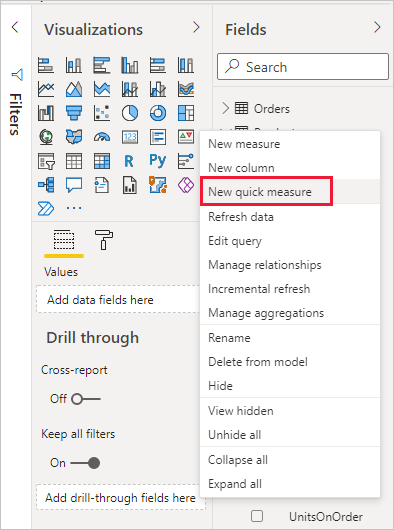
\includegraphics[width=\linewidth,height=4.4cm,keepaspectratio]{ms-learn/menu-medida-rapida.png}
    \column{0.36\textwidth}
    \centering
    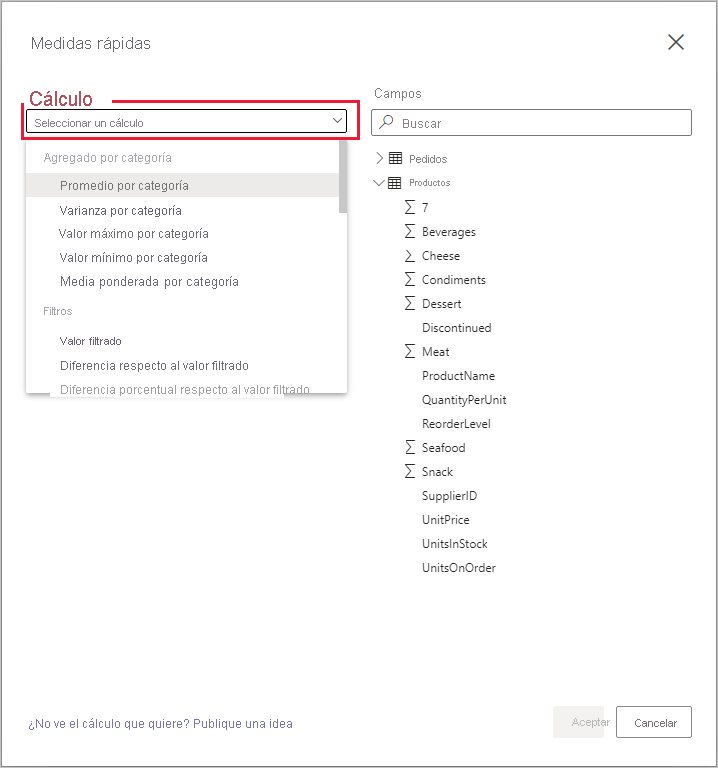
\includegraphics[width=\linewidth,height=4.1cm,keepaspectratio]{ms-learn/ventana-medidas-rapidas.png}
    \fuente{Uso de medidas rápidas para cálculos comunes}{\urlrapidas}
    \column{0.33\textwidth}
    \footnotesize
    Power BI también puede escribir la medida por ti:
    \begin{enumerate}
      \footnotesize
      \item Clic derecho en \texttt{Pagos} $>$ \menu{Nueva medida
        rápida}{New quick measure}.
      \item Elige un \menu{Cálculo}{Calculation} de la lista (por ejemplo,
        el cambio de mes a mes, en la categoría de inteligencia de tiempo)
        y arrastra los campos que pide.
      \item Power BI crea la medida y muestra su fórmula DAX.
    \end{enumerate}
    \scriptsize Úsalas para aprender: lee la fórmula que crearon y
    compárala con la del paso 2.
  \end{columns}
\end{frame}

\begin{frame}[t]{\npaso{4}\; Las metas}
  \small
  Un KPI necesita algo contra qué compararse. En una empresa, las metas
  vienen del plan del año; aquí las fijamos como dos medidas:
  \codigo{Meta de ingresos = 22000000\\[3pt]
    Meta de retención = 0.85}
  \small
  \begin{itemize}
    \small
    \item \texttt{Meta de ingresos}: 22 millones al mes. Créala en
      \texttt{Pagos}.
    \item \texttt{Meta de retención}: que el 85\% de los socios siga
      activo. Créala en \texttt{Socios} y dale formato de porcentaje.
  \end{itemize}
  \vspace{0.1cm}
  \begin{alertblock}{Una meta es una decisión de negocio}
    \footnotesize No la saques de los datos para que el KPI se vea bien:
    la pone quien dirige el negocio. Si no la tienes en tu proyecto,
    pregúntala o explica de dónde salió la que usaste.
  \end{alertblock}
\end{frame}

\begin{frame}[t]{\npaso{5}\; El objeto visual KPI: ingresos frente a la meta}
  \begin{columns}[T,onlytextwidth]
    \column{0.37\textwidth}
    \centering
    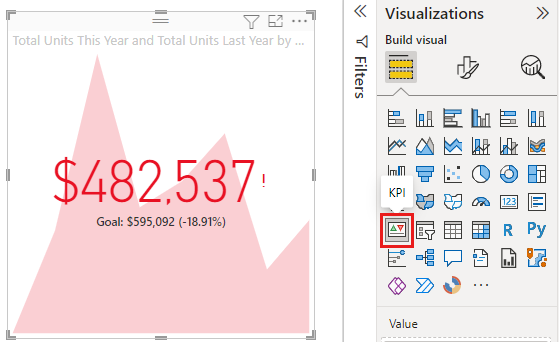
\includegraphics[width=\linewidth,height=2.4cm,keepaspectratio]{ms-learn/icono-kpi.png}
    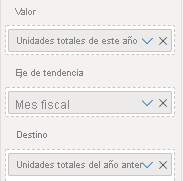
\includegraphics[width=0.48\linewidth,height=1.9cm,keepaspectratio]{ms-learn/kpi-casillas.png}
    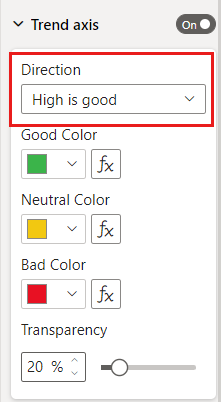
\includegraphics[width=0.48\linewidth,height=1.9cm,keepaspectratio]{ms-learn/kpi-direccion.png}
    \fuente{Visuales de indicador clave de rendimiento (KPI)}{\urlkpi}
    \column{0.6\textwidth}
    \footnotesize
    \begin{enumerate}
      \footnotesize
      \item Ícono \menu{KPI}{KPI} en Visualizaciones.
      \item \menu{Valor}{Value}: \texttt{Ingresos}. \menu{Eje de
        tendencia}{Trend axis}: \texttt{Calendario[Inicio de mes]}.
        \menu{Destino}{Target}: \texttt{Meta de ingresos}.
      \item En Formato $>$ \menu{Eje de tendencia}{Trend axis} $>$
        \menu{Dirección}{Direction}: \menu{Alto es bueno}{High is good}.
    \end{enumerate}
    \textbf{Debes ver}: \textbf{23.147.000}, el valor del último mes
    (septiembre de 2026), en verde, con la meta de 22.000.000 y una
    diferencia de \textbf{+5,2\%}. Al fondo, la tendencia de los meses.
    \begin{alertblock}{Por qué muestra solo el último mes}
      \scriptsize El KPI muestra el valor del último punto del eje de
      tendencia. Para ver otro mes, usa el segmentador del paso 7.
    \end{alertblock}
  \end{columns}
\end{frame}

\begin{frame}[t]{\npaso{6}\; Tarjetas: la variación y la retención}
  \small
  Dos tarjetas más, en la fila de los indicadores:
  \begin{enumerate}
    \small
    \item \menu{Tarjeta}{Card} con \texttt{Variación mensual}.
    \item \menu{Tarjeta}{Card} con \texttt{Porcentaje activos} y
      \texttt{Meta de retención}.
  \end{enumerate}
  \vspace{0.05cm}
  \begin{columns}[T,onlytextwidth]
    \column{0.48\textwidth}
    \footnotesize\textbf{Sin segmentadores, debes ver}:
    \begin{itemize}
      \footnotesize
      \item Variación mensual: \textbf{en blanco}. Sin un único mes elegido
        no hay ``mes anterior'' que comparar (por eso el
        \texttt{HASONEVALUE}). Se llena en el paso 7.
      \item Porcentaje activos: \textbf{80,0\%}, por debajo de la meta del
        85\%.
    \end{itemize}
    \column{0.48\textwidth}
    \begin{alertblock}{Una tarjeta sin meta no es un KPI}
      \scriptsize ``80\%'' solo no dice si es bueno o malo. Junto a la
      meta (85\%), dice que faltan 5 puntos: ahí empieza la pregunta de
      dónde actuar.
    \end{alertblock}
  \end{columns}
  \guia{Crear un visual de tarjeta en Power BI}{\urltarjeta}
\end{frame}

% ============================================================
\section{Hora 2: Segmentadores, filtros y jerarquías}
% ============================================================
\begin{frame}[t]{Segmentador o filtro: ¿quién decide?}
  \footnotesize
  \renewcommand{\arraystretch}{1.25}
  \begin{tabular}{@{}L{2.8cm}L{5.1cm}L{5.1cm}@{}}
    \toprule
    & \textbf{Segmentador} & \textbf{Filtro (panel Filtros)} \\
    \midrule
    ¿Quién lo cambia? & quien lee el tablero & quien diseña el tablero (o quien lee, si se lo permites) \\
    ¿Dónde se ve? & en la página, como botones o lista & en el panel Filtros, a un lado \\
    ¿Qué filtra? & la página (o varias, si los sincronizas) & un objeto visual, una página o todas las páginas \\
    Úsalo para & las preguntas que quien lee quiere responder: qué mes, qué sede & lo que debe quedar fijo: qué año muestra la página, quitar datos de prueba \\
    \bottomrule
  \end{tabular}

  \vspace{0.2cm}
  \small Regla práctica: si quien lee debería poder cambiarlo, es un
  segmentador. Si cambiarlo haría que la página dejara de responder su
  pregunta, es un filtro.
  \guia{Introducción a las segmentaciones en Power BI}{\urlsegmentadores}
\end{frame}

\begin{frame}[t]{\npaso{7}\; Segmentador del mes}
  \begin{columns}[T,onlytextwidth]
    \column{0.26\textwidth}
    \centering
    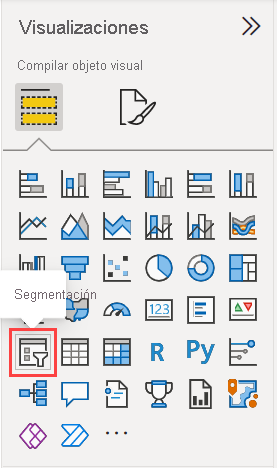
\includegraphics[width=\linewidth,height=4.2cm,keepaspectratio]{ms-learn/icono-segmentacion.png}
    \fuente{Tutorial: del modelo dimensional al informe}{\urltutorial}
    \column{0.71\textwidth}
    \footnotesize
    \begin{enumerate}
      \footnotesize
      \item Ícono \menu{Segmentación}{Slicer}. Campo: \texttt{Calendario[Año-Mes]}.
      \item En Formato $>$ \menu{Configuración de segmentación}{Slicer
        settings}: estilo \menu{Lista desplegable}{Dropdown} y
        \menu{Selección única}{Single select}.
      \item Elige \texttt{2026-09}.
    \end{enumerate}
    \textbf{Debes ver}, con el mes 2026-09:

    \scriptsize
    \begin{tabular}{@{}lr@{}}
      \toprule
      Ingresos & 23.147.000 \\
      Ingresos mes anterior & 22.932.000 \\
      Variación mensual & +0,94\% \\
      Visitas & 2428 \\
      \bottomrule
    \end{tabular}
    \vspace{0.05cm}

    \footnotesize Para elegir un rango de fechas en lugar de un mes, usa
    \texttt{Calendario[Date]} con el estilo \menu{Entre}{Between}. Pero
    la variación mensual compara un solo mes: con un rango, compara contra
    el mes anterior al inicio del rango.
    \guia{Visual de segmentación de datos}{\urlsegvisual}
  \end{columns}
\end{frame}

\begin{frame}[t]{\npaso{8}\; Segmentador de sede: elige bien la columna}
  \small
  \begin{enumerate}
    \small
    \item Otro \menu{Segmentación}{Slicer} con
      \textbf{\texttt{Socios[sede\_principal]}}, estilo
      \menu{Lista vertical}{Vertical list}.
  \end{enumerate}
  \begin{alertblock}{¿Por qué no Sedes[sede]?}
    \footnotesize Recuerda la estrella de la Clase 13: \texttt{Sedes} filtra
    \texttt{Pagos} y \texttt{Asistencias}, pero \textbf{no está relacionada
    con Socios}. Con \texttt{Sedes[sede]}, la tarjeta de porcentaje activos
    no cambiaría al elegir una sede, y la página mostraría cifras de
    universos distintos. \texttt{Socios[sede\_principal]} filtra a los
    socios, y a través de ellos a sus pagos y sus visitas: las tres cosas
    a la vez.
  \end{alertblock}
  \footnotesize\textbf{Debes ver}, con el mes 2026-09 y la Sede Poblado:
  Ingresos 8.017.000; Ingresos mes anterior 10.211.000; Variación mensual
  \textbf{$-$21,5\%}. Porcentaje activos 82,9\%.
  \vspace{0.05cm}

  \footnotesize Eso es un hallazgo: el gimnasio crece en septiembre
  (+0,94\%), pero Poblado cae. Lo investigamos en la diapositiva
  siguiente.
\end{frame}

\begin{frame}[t]{¿Por qué cae Poblado en septiembre?}
  \small
  Antes de decir ``Poblado está perdiendo socios'', valida (Clase 14):
  \vspace{0.1cm}
  \begin{columns}[T,onlytextwidth]
    \column{0.5\textwidth}
    \footnotesize Una tabla con \texttt{Planes[plan]} e \texttt{Ingresos},
    con los segmentadores en Poblado, y cambiando el mes:

    \vspace{0.05cm}
    \scriptsize
    \begin{tabular}{@{}lrr@{}}
      \toprule
      \textbf{Plan} & \textbf{2026-08} & \textbf{2026-09} \\
      \midrule
      Mensual & 4.851.000 & 4.761.000 \\
      Trimestral & 2.160.000 & 1.656.000 \\
      Anual & 3.200.000 & 1.600.000 \\
      \midrule
      \textbf{Total} & \textbf{10.211.000} & \textbf{8.017.000} \\
      \bottomrule
    \end{tabular}
    \column{0.47\textwidth}
    \footnotesize\textbf{Lectura}: el plan Mensual casi no cambia. La caída
    viene del plan Anual: en agosto hubo cuatro pagos anuales y en
    septiembre, dos. Los planes largos se pagan de una vez, así que los
    ingresos de un mes suben y bajan según cuántos se renuevan ese mes.
  \end{columns}
  \vspace{0.15cm}
  \begin{exampleblock}{El insight}
    \footnotesize La caída de Poblado en septiembre no es una pérdida de
    socios: es el calendario de pagos anuales. Recomendación: comparar
    los ingresos de los planes largos por trimestre o año, no mes a mes, y
    seguir de cerca solo el plan Mensual como señal de demanda.
  \end{exampleblock}
\end{frame}

\begin{frame}[t]{\npaso{9}\; Segmentador de grupo de edad}
  \small
  \begin{enumerate}
    \small
    \item Un tercer \menu{Segmentación}{Slicer} con
      \texttt{Socios[grupo\_edad]}.
    \item Quita la selección de mes y de sede (el borrador en la esquina de
      cada segmentador) y prueba cada grupo.
  \end{enumerate}
  \vspace{0.05cm}
  \begin{columns}[T,onlytextwidth]
    \column{0.5\textwidth}
    \footnotesize\textbf{Debes ver} (todo el periodo):

    \vspace{0.05cm}
    \scriptsize
    \begin{tabular}{@{}lrrr@{}}
      \toprule
      \textbf{Grupo} & \textbf{Socios} & \textbf{Activos} & \textbf{Ingresos} \\
      \midrule
      Joven (<=25) & 56 & 82,1\% & 36.316.000 \\
      Adulto (26-45) & 173 & 80,3\% & 111.378.000 \\
      Mayor (46+) & 71 & 77,5\% & 44.730.000 \\
      \bottomrule
    \end{tabular}
    \column{0.47\textwidth}
    \footnotesize\textbf{Lectura}: los tres grupos están por debajo de la
    meta de retención (85\%), y la diferencia entre ellos es pequeña: la
    edad no parece ser lo que separa a quienes se quedan. La distancia a la
    sede (Clase 14) separa mucho más.
  \end{columns}
  \vspace{0.1cm}
  \scriptsize Los segmentadores se combinan: elegir Poblado y Mayor muestra
  solo a los socios mayores de Poblado.
\end{frame}

\begin{frame}[t]{\npaso{10}\; Filtros de objeto visual y de página}
  \begin{columns}[T,onlytextwidth]
    \column{0.3\textwidth}
    \centering
    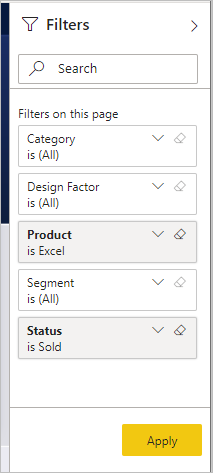
\includegraphics[width=\linewidth,height=3.6cm,keepaspectratio]{ms-learn/panel-filtros.png}
    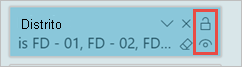
\includegraphics[width=\linewidth,height=0.9cm,keepaspectratio]{ms-learn/filtro-bloquear.png}
    \fuente{Dar formato a los filtros en informes de Power BI}{\urlformatofiltros}
    \column{0.67\textwidth}
    \footnotesize
    El panel \menu{Filtros}{Filters} tiene tres zonas: \textbf{en este
    objeto visual}, \textbf{en esta página} y \textbf{en todas las
    páginas}. Arrastra el campo a la zona que corresponda.
    \begin{enumerate}
      \footnotesize
      \item \textbf{Filtro de página}: arrastra \texttt{Calendario[Año]} a
        \menu{Filtros en esta página}{Filters on this page} y marca 2026.
        La página queda dedicada a 2026. Sin mes elegido, la tarjeta de
        ingresos muestra \textbf{164.884.000}.
      \item \textbf{Filtro de objeto visual}: en las barras de ingresos por
        sede, arrastra \texttt{Socios[sede\_principal]} a
        \menu{Filtros en este objeto visual}{Filters on this visual}, tipo
        \menu{N superior}{Top N}, 3, por \texttt{Ingresos}: quedan las tres
        sedes que más generan.
      \item El candado bloquea un filtro y el ojo lo oculta, para que quien
        lee no lo cambie.
    \end{enumerate}
    \guia{Tipos de filtros en informes de Power BI}{\urltiposfiltros}
  \end{columns}
\end{frame}

\begin{frame}[t]{\npaso{11}\; Una jerarquía: de departamento a barrio}
  \begin{columns}[T,onlytextwidth]
    \column{0.22\textwidth}
    \centering
    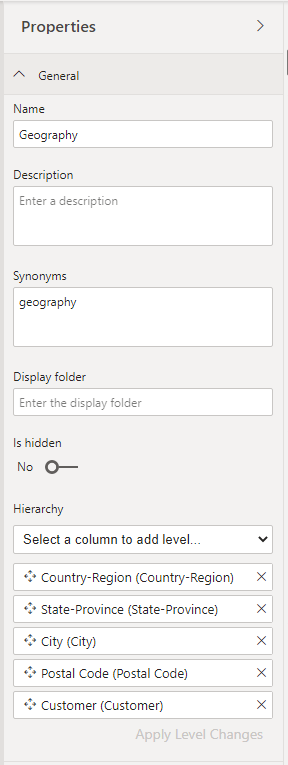
\includegraphics[width=\linewidth,height=4.3cm,keepaspectratio]{ms-learn/propiedades-jerarquia.png}
    \column{0.3\textwidth}
    \centering
    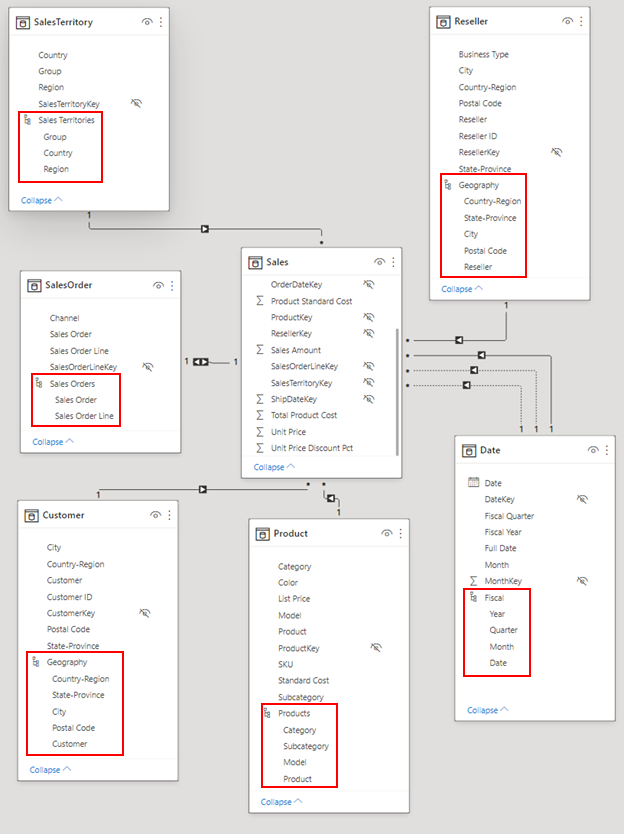
\includegraphics[width=\linewidth,height=3.9cm,keepaspectratio]{ms-learn/modelo-jerarquias.png}
    \fuente{Tutorial: del modelo dimensional al informe}{\urltutorial}
    \column{0.45\textwidth}
    \footnotesize
    \texttt{Socios} tiene la ubicación de lo general a lo particular. Una
    jerarquía junta esas columnas en ese orden:
    \begin{enumerate}
      \footnotesize
      \item En el panel Datos, clic derecho en \texttt{departamento} $>$
        \menu{Crear jerarquía}{Create hierarchy}.
      \item En el panel \menu{Propiedades}{Properties}, agrega los niveles
        \texttt{municipio} y \texttt{barrio}, en ese orden, y selecciona
        \menu{Aplicar cambios en el nivel}{Apply level changes}.
      \item Cámbiale el nombre a \texttt{Geografía}.
    \end{enumerate}
    \scriptsize Los niveles de una jerarquía deben estar en la misma
    tabla. A la izquierda, cómo se ven en la vista Modelo las jerarquías
    del ejemplo de Microsoft.
  \end{columns}
\end{frame}

\begin{frame}[t]{\npaso{12}\; Explorar en profundidad}
  \begin{columns}[T,onlytextwidth]
    \column{0.45\textwidth}
    \centering
    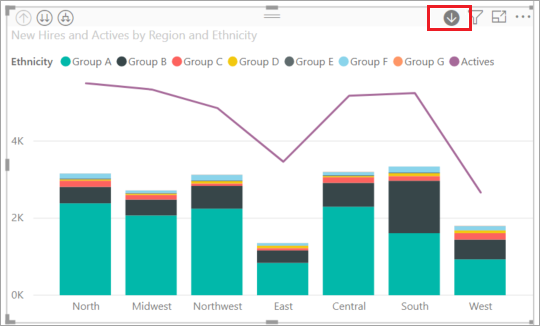
\includegraphics[width=\linewidth,height=2.7cm,keepaspectratio]{ms-learn/explorar-profundidad.png}
    \fuente{Cambiar cómo interactúan los objetos visuales}{\urlinteracciones}
    \vspace{0.05cm}
    \footnotesize\raggedright\textbf{Debes ver}: Antioquia 197 socios (80,7\%
    activos), Bogotá, D.C. 82 (80,5\%), Valle del Cauca 21 (71,4\%). En
    Antioquia: Medellín 94, Sabaneta 39, Envigado 16, Caldas 16\ldots{} En
    Medellín: El Poblado 29, Laureles 24, Belén 22, Robledo 15.
    \column{0.52\textwidth}
    \footnotesize
    \begin{enumerate}
      \footnotesize
      \item \menu{Gráfico de barras agrupadas}{Clustered bar chart}, con la
        jerarquía \texttt{Geografía} en el Eje Y, \texttt{Socios} en el Eje
        X y \texttt{Porcentaje activos} en
        \menu{Información sobre herramientas}{Tooltips}.
      \item Activa la flecha hacia abajo de la parte superior del objeto
        visual (modo de exploración). Haz clic en \textit{Antioquia}: ves
        sus municipios. Clic en \textit{Medellín}: ves sus barrios.
      \item La flecha hacia arriba sube un nivel.
    \end{enumerate}
    \begin{alertblock}{Una jerarquía de fechas también sirve}
      \scriptsize Crea \texttt{Año} $>$ \texttt{Mes} $>$ \texttt{Date} en
      \texttt{Calendario} y úsala en una línea: pasas de años a meses y a
      días con la misma flecha.
    \end{alertblock}
    \guia{Usar el modo de exploración en profundidad}{\urlexplorar}
  \end{columns}
\end{frame}

% ============================================================
\section{Hora 3: Interacción y diseño de la página}
% ============================================================
\begin{frame}[t]{\npaso{13}\; Interacción entre objetos visuales}
  \begin{columns}[T,onlytextwidth]
    \column{0.47\textwidth}
    \centering
    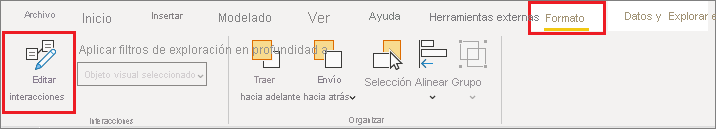
\includegraphics[width=\linewidth,height=1.3cm,keepaspectratio]{ms-learn/editar-interacciones.png}
    \fuente{Cambiar cómo interactúan los objetos visuales}{\urlinteracciones}
    \vspace{0.1cm}
    \footnotesize\raggedright Al hacer clic en una barra, los demás objetos
    visuales de la página reaccionan. Hay tres opciones para cada uno:
    \begin{itemize}
      \scriptsize
      \item \textbf{Filtrar}: muestra solo lo de esa barra.
      \item \textbf{Resaltar}: muestra todo, y destaca la parte de esa
        barra.
      \item \textbf{Ninguno}: no cambia.
    \end{itemize}
    \column{0.5\textwidth}
    \footnotesize
    \begin{enumerate}
      \footnotesize
      \item Selecciona las barras de \texttt{Geografía} y ve a
        \menu{Formato}{Format} $>$ \menu{Editar interacciones}{Edit
        interactions}.
      \item Sobre el KPI de ingresos aparecen unos íconos pequeños: elige
        \textbf{Ninguno} (el círculo tachado).
      \item Repite con los segmentadores de sede y de grupo de edad: el KPI
        en \textbf{Ninguno}. Deja el del mes en \textbf{Filtrar}.
      \item Vuelve a hacer clic en \menu{Editar
        interacciones}{Edit interactions} para terminar.
    \end{enumerate}
    \textbf{Por qué}: la meta de 22 millones es de todo el gimnasio. Filtrado
    por sede, el KPI compararía una parte contra la meta del todo. Las
    tarjetas sí se filtran: la meta del 85\% vale para cada sede.
  \end{columns}
\end{frame}

\begin{frame}[t]{\npaso{14}\; Ordenar la página}
  \small
  \begin{enumerate}
    \small
    \item \menu{Vista}{View} $>$ activa \menu{Líneas de
      cuadrícula}{Gridlines} y \menu{Ajustar a la cuadrícula}{Snap to
      grid}: los objetos visuales se alinean solos.
    \item Ubica las zonas como en el boceto: título arriba, indicadores en
      una fila, segmentadores a la izquierda, gráficos debajo.
    \item Usa el mismo ancho y alto en los objetos visuales de una misma
      fila.
    \item Revisa que cada color signifique lo mismo en toda la página
      (Clase 14).
  \end{enumerate}
  \vspace{0.1cm}
  \begin{columns}[T,onlytextwidth]
    \column{0.48\textwidth}
    \begin{exampleblock}{De lo general a lo particular}
      \footnotesize Se lee como un texto: de arriba a la izquierda hacia
      abajo a la derecha. Primero ``cómo vamos'' (KPI), después ``dónde''
      (sede, geografía).
    \end{exampleblock}
    \column{0.48\textwidth}
    \begin{alertblock}{Menos es más}
      \footnotesize Entre cinco y ocho objetos visuales por página. Si
      necesitas más, haz otra página con su propia pregunta.
    \end{alertblock}
  \end{columns}
  \guia{Uso de líneas de cuadrícula y ajuste a la cuadrícula}{\urlcuadricula}
\end{frame}

\begin{frame}[t]{\npaso{15}\; Prueba la página como si no la conocieras}
  \small
  Antes de entregarla, haz estas pruebas:
  \vspace{0.05cm}
  \begin{enumerate}
    \small
    \item \textbf{Los cinco segundos} (Clase 11): muéstrasela a alguien
      durante cinco segundos. ¿Puede decirte cómo va el gimnasio?
    \item \textbf{Cada segmentador}: cambia cada uno y mira que todos los
      indicadores reaccionen. Si uno no cambia, revisa qué columna usa el
      segmentador (paso 8) o sus interacciones (paso 13).
    \item \textbf{Los totales}: sin segmentadores, ¿las cifras coinciden
      con las de la Clase 14?
    \item \textbf{Los blancos}: una tarjeta en blanco confunde. Si la
      variación mensual está en blanco sin mes elegido, agrega en su título
      ``elige un mes''.
  \end{enumerate}
  \vspace{0.1cm}
  \begin{exampleblock}{La pregunta de fondo}
    \footnotesize ¿Quien lee la página puede responder, solo, la pregunta del
    título y decidir dónde actuar? Si necesita que tú le expliques, la
    página todavía no está lista.
  \end{exampleblock}
\end{frame}

\begin{frame}[t]{Checklist: la página está lista cuando\ldots}
  \small
  \begin{enumerate}
    \item El título dice qué pregunta de negocio responde la página.
    \item Cada indicador tiene una meta o un punto de comparación.
    \item Los segmentadores filtran todos los indicadores, y usan columnas
      de la tabla correcta.
    \item Lo que debe quedar fijo está en un filtro, bloqueado si hace
      falta.
    \item Las interacciones tienen sentido: nada compara una parte contra
      una meta del todo.
    \item Hay entre cinco y ocho objetos visuales, alineados, con colores
      coherentes.
    \item Sin segmentadores, los totales coinciden con los de la Clase 14.
  \end{enumerate}
\end{frame}

% ============================================================
\section{Taller}
% ============================================================
\begin{frame}[t]{Actividad práctica}
  \begin{columns}[T,onlytextwidth]
    \column{0.48\textwidth}
    \begin{block}{Parte A: el gimnasio (en clase)}
      \small Construye la página \texttt{Resumen} de los pasos 1 a 15 y
      comprueba cada cifra de la guía.
    \end{block}
    \column{0.48\textwidth}
    \begin{alertblock}{Parte B: tu proyecto}
      \small La primera página de tu tablero:
      \begin{enumerate}
        \footnotesize
        \item Escribe la pregunta de negocio que responde.
        \item Al menos dos indicadores con meta (KPI o tarjeta).
        \item Al menos dos segmentadores que funcionen en todos los
          objetos visuales.
        \item Un filtro de página o de objeto visual, y una jerarquía si
          tus datos la tienen.
        \item Actualiza tu ficha de insights con lo que revelaron los
          segmentadores.
      \end{enumerate}
    \end{alertblock}
  \end{columns}
\end{frame}

\begin{frame}[t]{Producto esperado}
  \begin{exampleblock}{Entregable}
    \small
    \begin{enumerate}
      \item El archivo \texttt{.pbix} de tu proyecto, con la página del
        tablero terminada.
      \item Dos capturas de esa página: sin segmentadores y con una
        selección que muestre un hallazgo (en Windows: tecla Windows + Mayús
        + S).
      \item La ficha de insights actualizada (Clase 14), con al menos un
        insight que salió de usar los segmentadores.
    \end{enumerate}
  \end{exampleblock}
  \small Este tablero es la base de la Clase 16 (MasterClass), donde
  repasamos el Módulo 3 y preparamos el bootcamp.
\end{frame}

% ============================================================
\section{Cierre}
% ============================================================
\begin{frame}[t]{Cierre y próxima sesión}
  \begin{itemize}
    \item Una medida se calcula de nuevo según los filtros de cada lugar
      donde está: es el \texttt{groupby} de Power BI.
    \item Un KPI compara contra una meta; sin meta, un número no dice si
      algo va bien.
    \item Los segmentadores son para quien lee; los filtros, para quien
      diseña. Y deben usar columnas que filtren todo lo que muestra la
      página.
    \item Un segmentador puede revelar lo que el total esconde, como la
      caída de Poblado; antes de concluir, se valida.
    \item Próxima sesión, \textbf{Clase 16: MasterClass} (presencial):
      recapitulación del Módulo 3 y preparación del bootcamp.
  \end{itemize}
\end{frame}

\begin{frame}[t]{Documentación oficial usada en cada paso}
  \scriptsize
  Todas las páginas son de Microsoft Learn, en español. Haz clic en el
  título para abrirla.
  \vspace{0.1cm}
  \renewcommand{\arraystretch}{1.08}
  \begin{columns}[T,onlytextwidth]
    \column{0.49\textwidth}
    \begin{tabular}{@{}L{1.4cm}L{4.95cm}@{}}
      \toprule
      \textbf{Paso} & \textbf{Página oficial} \\
      \midrule
      1 y 14 & \href{\urltrucos}{\color{esumerOrange}Sugerencias para crear informes} y \href{\urlcuadricula}{\color{esumerOrange}líneas de cuadrícula} \\
      2 & \href{\urlmedidas}{\color{esumerOrange}Medidas}; \href{https://learn.microsoft.com/es-es/dax/calculate-function-dax}{\color{esumerOrange}CALCULATE}, \href{https://learn.microsoft.com/es-es/dax/previousmonth-function-dax}{\color{esumerOrange}PREVIOUSMONTH}, \href{https://learn.microsoft.com/es-es/dax/divide-function-dax}{\color{esumerOrange}DIVIDE}, \href{https://learn.microsoft.com/es-es/dax/all-function-dax}{\color{esumerOrange}ALL} y \href{https://learn.microsoft.com/es-es/dax/hasonevalue-function-dax}{\color{esumerOrange}HASONEVALUE} \\
      3 & \href{\urlrapidas}{\color{esumerOrange}Medidas rápidas} \\
      5 & \href{\urlkpi}{\color{esumerOrange}Objeto visual KPI} \\
      6 & \href{\urltarjeta}{\color{esumerOrange}Objeto visual de tarjeta} \\
      \bottomrule
    \end{tabular}
    \column{0.49\textwidth}
    \begin{tabular}{@{}L{1.4cm}L{4.95cm}@{}}
      \toprule
      \textbf{Paso} & \textbf{Página oficial} \\
      \midrule
      7 a 9 & \href{\urlsegmentadores}{\color{esumerOrange}Introducción a las segmentaciones} y \href{\urlsegvisual}{\color{esumerOrange}visual de segmentación} \\
      10 & \href{\urltiposfiltros}{\color{esumerOrange}Tipos de filtros}, \href{\urlfiltros}{\color{esumerOrange}agregar un filtro} y \href{\urlformatofiltros}{\color{esumerOrange}formato del panel} \\
      11 & \href{\urltutorial}{\color{esumerOrange}Tutorial: del modelo dimensional al informe} \\
      12 & \href{\urlexplorar}{\color{esumerOrange}Exploración en profundidad} y \href{\urlsegjerarquia}{\color{esumerOrange}segmentador con jerarquía} \\
      13 & \href{\urlinteracciones}{\color{esumerOrange}Interacción entre objetos visuales} \\
      Diseño & \href{\urltemas}{\color{esumerOrange}Temas de informe} \\
      \bottomrule
    \end{tabular}
  \end{columns}
\end{frame}

\begin{frame}[t]{Para seguir aprendiendo}
  \footnotesize
  \begin{columns}[T,onlytextwidth]
    \column{0.52\textwidth}
    \textbf{Módulos de Microsoft Learn, en español}
    \begin{itemize}
      \footnotesize
      \item \href{https://learn.microsoft.com/es-es/training/modules/dax-power-bi-modify-filter/}{\color{esumerOrange}Modificar el contexto de filtro en DAX} (CALCULATE)
      \item \href{https://learn.microsoft.com/es-es/training/modules/dax-power-bi-time-intelligence/}{\color{esumerOrange}Funciones de inteligencia de tiempo de DAX}
      \item \href{https://learn.microsoft.com/es-es/training/modules/power-bi-effective-reports/}{\color{esumerOrange}Diseñar informes de Power BI}
      \item \href{https://learn.microsoft.com/es-es/training/modules/visuals-in-power-bi/}{\color{esumerOrange}Diseño de informes eficaces en Power BI}
    \end{itemize}
    \column{0.45\textwidth}
    \textbf{Descargas}
    \begin{itemize}
      \footnotesize
      \item \href{\urlstore}{\color{esumerOrange}Power BI Desktop en Microsoft Store}
      \item \href{\urlcentro}{\color{esumerOrange}Power BI Desktop en el Centro de descargas}
      \item \href{\urldatos}{\color{esumerOrange}Datos de la clase: gimnasio\_vitalis.xlsx}
    \end{itemize}
    \textbf{De este curso}
    \begin{itemize}
      \footnotesize
      \item Clase 9: \texttt{groupby}, la idea detrás de las medidas.
      \item Clase 13: el modelo estrella y sus relaciones.
      \item Clase 14: validar cifras y la ficha de insights.
    \end{itemize}
  \end{columns}
\end{frame}

\begin{frame}[t]{Créditos de las imágenes}
  \scriptsize
  Las capturas de pantalla de Microsoft Power BI Desktop provienen de la
  documentación de Microsoft Learn y se reproducen sin modificaciones,
  conforme a la política de Microsoft sobre capturas de pantalla de sus
  productos. \textbf{Used with permission from Microsoft.}
  \vspace{0.15cm}

  Páginas de origen:
  \begin{itemize}
    \scriptsize
    \item \href{\urlrapidas}{Uso de medidas rápidas para cálculos comunes y eficaces}
      \textperiodcentered\ \href{\urlkpi}{Visuales de indicador clave de rendimiento (KPI)}
    \item \href{\urltutorial}{Tutorial: Del modelo dimensional al informe impresionante en Power BI Desktop}
      \textperiodcentered\ \href{\urlformatofiltros}{Dar formato a los filtros en informes de Power BI}
    \item \href{\urlinteracciones}{Cambiar cómo interactúan los objetos visuales en un informe}
  \end{itemize}
  \vspace{0.1cm}
  Los datos del Gimnasio Vitalis son ficticios, creados para el curso.
  Las metas de ingresos y de retención son supuestos de práctica.
\end{frame}

{
\setbeamertemplate{footline}{}
\begin{frame}[plain,noframenumbering]
  \begin{tikzpicture}[remember picture,overlay]
    \fill[esumerNavy] (current page.south west) rectangle (current page.north east);
    \node at (current page.center) {\color{white}\Huge\bfseries ¡Gracias!};
  \end{tikzpicture}
\end{frame}
}

\end{document}
